\documentclass{beamer}
\usepackage{amsmath}
\usepackage[english]{babel} %set language; note: after changing this, you need to delete all auxiliary files to recompile
\usepackage[utf8]{inputenc} %define file encoding; latin1 is the other often used option
\usepackage{csquotes} % provides context sensitive quotation facilities
\usepackage{graphicx} %allows for inserting figures
\usepackage{booktabs} % for table formatting without vertical lines
\usepackage{textcomp} % allow for example using the Euro sign with \texteuro
\usepackage{stackengine}
\usepackage{wasysym}
\usepackage{tikzsymbols}
\usepackage{textcomp}
\usepackage{ragged2e} % para alinear
\usepackage{graphicx}  % Para incluir imágenes
\usepackage{tikz}  
\usepackage{booktabs}
\usepackage{colortbl}
\usepackage{xcolor}
\usepackage{array}
\usepackage{wrapfig}
% ELIMINAR COMANDOS DE NAVEGACION%%%%%%%%%%%
\setbeamertemplate{navigation symbols}

%\newcommand{\bubblethis}[2]{
 %       \tikz[remember picture,baseline]{\node[anchor=base,inner sep=0,outer sep=0]%
 %       (#1) {\underline{#1}};\node[overlay,cloud callout,callout relative pointer={(0.2cm,-0.7cm)},%
 %       aspect=2.5,fill=yellow!90] at ($(#1.north)+(-0.5cm,1.6cm)$) {#2};}%
 %   }%
%\tikzset{face/.style={shape=circle,minimum size=4ex,shading=radial,outer sep=0pt,
 %       inner color=white!50!yellow,outer color= yellow!70!orange}}

%% Some commands to make the code easier
\newcommand{\emoticon}[1][]{%
  \node[face,#1] (emoticon) {};
  %% The eyes are fixed.
  \draw[fill=white] (-1ex,0ex) ..controls (-0.5ex,0.2ex)and(0.5ex,0.2ex)..
        (1ex,0.0ex) ..controls ( 1.5ex,1.5ex)and( 0.2ex,1.7ex)..
        (0ex,0.4ex) ..controls (-0.2ex,1.7ex)and(-1.5ex,1.5ex)..
        (-1ex,0ex)--cycle;}
\newcommand{\pupils}{
  %% standard pupils
  \fill[shift={(0.5ex,0.5ex)},rotate=80] 
       (0,0) ellipse (0.3ex and 0.15ex);
  \fill[shift={(-0.5ex,0.5ex)},rotate=100] 
       (0,0) ellipse (0.3ex and 0.15ex);}

\newcommand{\emoticonname}[1]{
  \node[below=1ex of emoticon,font=\footnotesize,
        minimum width=4cm]{#1};}
\usepackage{scalerel}
\usetikzlibrary{positioning}
\usepackage{xcolor,amssymb}
\newcommand\dangersignb[1][2ex]{%
  \scaleto{\stackengine{0.3pt}{\scalebox{1.1}[.9]{%
  \color{red}$\blacktriangle$}}{\tiny\bfseries !}{O}{c}{F}{F}{L}}{#1}%
}
\newcommand\dangersignw[1][2ex]{%
  \scaleto{\stackengine{0.3pt}{\scalebox{1.1}[.9]{%
  \color{red}$\blacktriangle$}}{\color{white}\tiny\bfseries !}{O}{c}{F}{F}{L}}{#1}%
}
\usepackage{fontawesome} % Social Icons
\usepackage{epstopdf} % allow embedding eps-figures
\usepackage{tikz} % allows drawing figures
\usepackage{amsmath,amssymb,amsthm} %advanced math facilities
\usepackage{lmodern} %uses font that support italic and bold at the same time

\usepackage{tikz}

\usepackage{tcolorbox}



\usefonttheme[onlymath]{serif} %set math font to serif ones

\definecolor{beamerblue}{rgb}{0.2,0.2,0.7} %define beamerblue color for later use

%%% defines highlight command to set text blue
\newcommand{\highlight}[1]{{\color{blue}{#1}}}


%%%%%%% commands defining backup slides so that frame numbering is correct
\newtcolorbox{boxA}{
    fontupper = \bf,
    boxrule = 1.5pt,
    colframe = black % frame color
}
\newtcolorbox{boxB}{
    boxrule = 1.5pt,
    colframe = blue!70!black,, % frame color
    colback = blue!7!white,
}
\newcommand{\backupbegin}{
   \newcounter{framenumberappendix}
   \setcounter{framenumberappendix}{\value{framenumber}}
}
\newcommand{\backupend}{
   \addtocounter{framenumberappendix}{-\value{framenumber}}
   \addtocounter{framenumber}{\value{framenumberappendix}}
}

%%%% end of defining backup slides

%Specify figure caption, see also http://tex.stackexchange.com/questions/155738/caption-package-not-working-with-beamer
\setbeamertemplate{caption}{\insertcaption} %redefines caption to remove label "Figure".
%\setbeamerfont{caption}{size=\scriptsize,shape=\itshape,series=\bfseries} %sets figure  caption bold and italic and makes it smaller


\usetheme{Boadilla}
\usepackage{hyperref}
% --------------------
% Overall information
% --------------------
\title[Economía I]{Economía I \vspace{4mm}
\\ Magistral 3: Preferencias y utilidad}
\date{}
\author[Franco Riottini]{Franco Riottini}
\vspace{0.4cm}
\institute[]{Universidad de San Andrés} 

\begin{document}

\begin{frame}
\titlepage
\centering

\includegraphics[scale=0.2]{../Figures/logoUDESA.jpg} 
\end{frame}

\begin{frame}{Las preferencias del estudiante}
    \begin{itemize}
        \item Hasta ahora vimos que nuestros ingresos imponen una restricción que puede influir en nuestra elección de consumo. \vspace{2mm}
        \begin{itemize}
        \item Cuando tenemos que decidir qué canasta queremos consumir, debemos limitarnos a elegir entre todas las canastas \textbf{alcanzables}.  \vspace{3mm}
        \end{itemize}
        \item ¿Qué nos falta para resolver el problema del consumidor?  \vspace{2mm}
        \begin{itemize}
        \item Necesitamos identificar qué \textbf{prefiere} entre todas las canastas que se pueden alcanzar.
        \end{itemize}
    \end{itemize}
\end{frame}

\begin{frame}{Las preferencias del estudiante}
    \begin{center}
    \begin{tikzpicture}
        % Ejes
        \draw[thick,->] (0,0) -- (6,0) node[below] {Pizza};
        \draw[thick,->] (0,0) -- (0,5.5) node[left] {Cerveza};
        % Imágenes
        \node at (0.7,4.5) {
\includegraphics[width=1.2cm]{../Figures/cerveza.png}};
        \node at (5,0.8) {
\includegraphics[width=1.5cm]{../Figures/pizza.jpg}};
        % Texto
        \node at (3.2,2.5) {\textbf{{\large ¿Cómo prefieren combinarlos?}}};
    \end{tikzpicture}
    \end{center}
\end{frame}

\begin{frame}{Tenemos distintas combinaciones...}
    Supongamos que tenemos un conjunto de canastas de pizza y cerveza. 
    \begin{center}
        \renewcommand{\arraystretch}{1.5} % Ajuste de altura de filas
        \setlength{\arrayrulewidth}{1pt} % Grosor de bordes
        \setlength{\tabcolsep}{10pt} % Espaciado en columnas
        \begin{tabular}{>{\bfseries}c|c|c}
            \textbf{\textcolor{blue}{Canasta}} & \textbf{\textcolor{blue}{Pizza}} & \textbf{\textcolor{blue}{Cerveza}} \\
            \hline
            A & 3  & 15  \\
            B & 5  & 11  \\
            C & 10 & 7   \\
            D & 15 & 5   \\
            E & 20 & 3   \\
            F & 15 & 11  \\
            G & 20 & 9   \\
            H & 15 & 15  \\
        \end{tabular}
    \end{center}
\end{frame}

\begin{frame}{...que podemos representar así}
    
    \begin{center}
        \begin{tikzpicture}[scale=0.6]
    
            \node at (14.5,5) {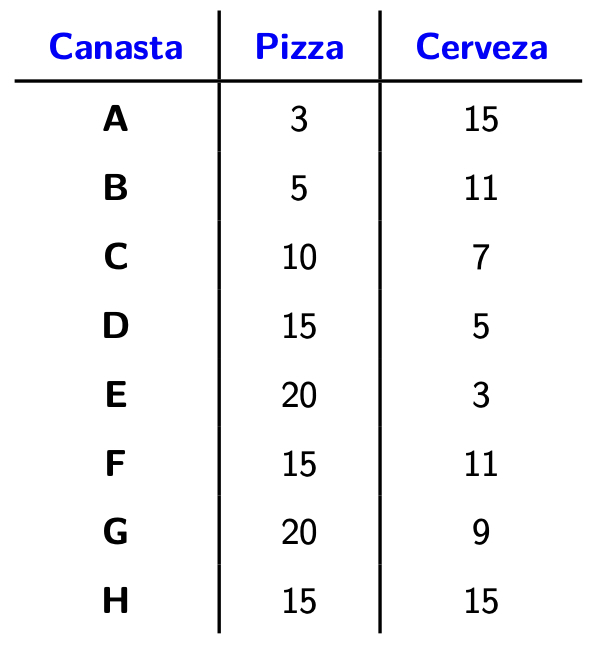
\includegraphics[width=3.5cm]{../Figures/tabla_canastas.jpg}};
    
            % Ejes
            \draw[thick,->] (0,0) -- (12,0) node[below right] {Pizza};
            \draw[thick,->] (0,0) -- (0,8.5) node[left] {Cerveza};
            
             % Etiquetas de cantidades de cerveza
            \node[left] at (0,7.5) {15};
            \node[left] at (0,5.5) {11};
            \node[left] at (0,4.5) {9};
            \node[left] at (0,3.5) {7};
            \node[left] at (0,2.5) {5};
            \node[left] at (0,1.5) {3};
    
            % Etiquetas de cantidades de pizza
            \node[below] at (1.5,0) {3};
            \node[below] at (2.5,0) {5};
            \node[below] at (5,0) {10};
            \node[below] at (7.5,0) {15};
            \node[below] at (10,0) {20};
    
            \only<2->{
            \draw[dashed] (0,7.5) -- (1.5,7.5);
            \draw[dashed] (1.5,7.5) --(1.5,0) ;
            \fill[red] (1.5,7.5) circle (2.5pt) node[above right] {A};
            }
            
            \only<3->{
            \draw[thick,->,blue] (1.5,7.5) -- (1.5,5.6);
            \draw[thick,->,blue] (1.5,5.5) -- (2.4,5.5);
            \draw[dashed] (0,5.5) -- (2.5,5.5);
            \draw[dashed] (2.5,5.5) --(2.5,0);
            \fill[black] (1.5,5.5) circle (2.5pt);
            \fill[red] (2.5,5.5) circle (2.5pt) node[above right] {B};
            \node[right,blue] at (1.4,6.5) {\scalebox{0.8}{4}};
            \node[above,blue] at (2,4.8) {\scalebox{0.8}{2}};
            }
    
            % Flechas indicando la TMT
            \only<4->{
            \draw[thick,->,blue] (2.5,5.5) -- (2.5,3.6);
            \draw[thick,->,blue] (2.5,3.5) -- (4.9,3.5);
            \draw[thick,->,blue] (5,3.5) -- (5,2.6);
            \draw[thick,->,blue] (5,2.5) -- (7.4,2.5);
            \draw[thick,->,blue] (7.5,2.5) -- (7.5,1.6);
            \draw[thick,->,blue] (7.5,1.5) -- (9.9,1.5);
    
            % Puntos clave en rojo
            \fill[black] (2.5,3.5) circle (2.5pt);
            \fill[red] (5,3.5) circle (2.5pt) node[above right] {C};
            \fill[black] (5,2.5) circle (2.5pt);
            \fill[black] (7.5,1.5) circle (2.5pt);
            \fill[red] (7.5,2.5) circle (2.5pt) node[above right] {D};
            \fill[red] (10,1.5) circle (2.5pt) node[above right] {E};
    
    
            % Etiquetas de TMT
            \node[right,blue] at (2.5,4.5) {\scalebox{0.8}{4}};
            \node[right,blue] at (4.9,3) {\scalebox{0.8}{2}};
            \node[above,blue] at (3.7,2.85) {\scalebox{0.8}{5}};
            \node[above,blue] at (6.3,1.85) {\scalebox{0.8}{5}};
            \node[above,blue] at (8.8,0.8) {\scalebox{0.8}{5}};
            
            % Líneas punteadas
            \draw[dashed] (0,3.5) -- (2.4,3.5);
            \draw[dashed] (0,2.5) --(4.9,2.5);
            \draw[dashed] (5,2.5) --(5,0);
            \draw[dashed] (0,1.5) --(7.4,1.5);
            \draw[dashed] (7.5,1.5) --(7.5,0);
            \draw[dashed] (10,1.5) --(10,0);
            }
            
             % F G y H
            \only<5->{
            \draw[dashed] (7.5,7.5) --(0,7.5);
            \draw[dashed] (7.5,7.5) --(7.5,0);
    
            \draw[dashed] (0,5.5) --(7.5,5.5);
            \draw[dashed] (0,4.5) --(10,4.5);
            \draw[dashed] (10,4.5) --(10,1.5);
            \fill[red] (7.5,7.5) circle (2.5pt) node[above right] {H};
            \fill[red] (7.5,5.5) circle (2.5pt) node[above right] {F};
            \fill[red] (10,4.5) circle (2.5pt) node[above right] {G};
            }
    
        \end{tikzpicture}
    \end{center}
\end{frame}
    
\begin{frame}{Algunas nos dejan igual de feliz}
    Supongamos que el estudiante revela que se encuentra indiferente entre las canastas A, B, C, D y E
    
    \begin{center}
        \begin{tikzpicture}[scale=0.6]
    
            % Ejes
            \draw[thick,->] (0,0) -- (12,0) node[below right] {Pizza};
            \draw[thick,->] (0,0) -- (0,8.5) node[left] {Cerveza};
            
             % Etiquetas de cantidades de cerveza
            \node[left] at (0,7.5) {15};
            \node[left] at (0,5.5) {11};
            \node[left] at (0,4.5) {9};
            \node[left] at (0,3.5) {7};
            \node[left] at (0,2.5) {5};
            \node[left] at (0,1.5) {3};
    
            % Etiquetas de cantidades de pizza
            \node[below] at (1.5,0) {3};
            \node[below] at (2.5,0) {5};
            \node[below] at (5,0) {10};
            \node[below] at (7.5,0) {15};
            \node[below] at (10,0) {20};
    
            % Puntos clave en rojo
            \fill[red] (1.5,7.5) circle (2.5pt) node[above right] {A};
            \fill[red] (2.5,5.5) circle (2.5pt) node[above right] {B};
            \fill[red] (5,3.5) circle (2.5pt) node[above right] {C};
            \fill[red] (7.5,2.5) circle (2.5pt) node[above right] {D};
            \fill[red] (10,1.8) circle (2.5pt) node[above right] {E};
    
             % F G y H
            \fill[red] (7.5,7.5) circle (2.5pt) node[above right] {H};
            \fill[red] (7.5,5.5) circle (2.5pt) node[above right] {F};
            \fill[red] (10,4.5) circle (2.5pt) node[above right] {G};
            
            % Curva de indiferencia
            \only<2->{
            \draw[thick, red] plot[smooth, tension=0.4] coordinates {(1.3,8) (1.5,7.5) (2.5,5.5) (3.5,4.5) (5,3.5) (7.5,2.5) (10,1.8) (11,1.6)};
            }
            \only<3->{
            \draw[thick, red] plot[smooth, tension=0.4] coordinates {(4.65,8) (5.1,7.5) (6.1,6.5) (7.5,5.5) (8.5,5) (10,4.5) (11,4.3)};
            }
            \only<4->{
            \draw[thick, red] plot[smooth, tension=0.4] coordinates {(7,8) (7.5,7.5) (8.5,7) (10,6.5) (11,6.3)};
            }
    
        \end{tikzpicture}
    \end{center}
\end{frame}

\begin{frame}{Las curvas de indiferencia}
    \begin{itemize}
        \item Todas las posibles canastas que otorgan el mismo nivel de utilidad o felicidad se encuentran sobre una misma \textbf{curva de indiferencia}. \vspace{2mm}
        \item ¿Qué nivel de felicidad nos dan esas canastas? 
        \begin{itemize}
        \item No nos interesa cuánto. Lo único relevante es si una canasta tiene una utilidad mayor a otra. 
        \item Vemos que las canastas F y G están sobre otra curva de indiferencia. Osea que nos dan otro nivel de utilidad. Lo mismo sucede con la canasta H. \vspace{1mm}
        \end{itemize}
        \item La cantidad de curvas de indiferencia podemos suponer que es \textbf{infinita}. Esto nos forma un \textbf{mapa de indiferencia}, donde las que están más a la derecha y arriba brindan más utilidad.
    \end{itemize}
\end{frame}

\begin{frame}{Supuestos de la relación de preferencias}
    \begin{enumerate}
    \item \textcolor{blue}{Completitud}: Los consumidores pueden \textbf{comparar} y \textbf{ordenar} cualquier par de canastas de bienes.
    \item \textcolor{blue}{Transitividad}: Si un consumidor prefiere la canasta A a la B y la B a la C, entonces prefiere la canasta A a la C.
        \begin{itemize}
            \item Las curvas de indiferencia no se cruzan
        \end{itemize}
    \item \textcolor{blue}{Monotonicidad fuerte}: Si una canasta tiene al menos una unidad más de un bien, entonces esa canasta es preferida. Esto implica que:
        \begin{itemize}
            \item Las curvas de indiferencia tienen pendiente negativa. 
            \item Las curvas de indiferencia más altas corresponden a niveles de utilidad más altos (más es mejor).
        \end{itemize}
    
    \item \textcolor{blue}{Convexidad}: Los consumidores prefieren consumir canastas de consumo \textit{balanceadas} antes que aquellas canastas que tienen mucho de un solo bien.
        \begin{itemize}
            \item Las curvas de indiferencia son convexas: se hacen más empinadas a la izquierda y más planas a la derecha 
        \end{itemize}
    \end{enumerate} 
\end{frame}


\begin{frame}
\frametitle{¿Qué es la utilidad marginal decreciente?}
\begin{itemize}
    \item Nos dice cómo cambia la utilidad total cuando agregamos una unidad adicional de un bien mientras dejamos constante la cantidad del otro bien 
    \item Esto podemos verlo relacionando la utilidad total con la cantidad de uno de los bienes que posee el consumidor    
\end{itemize}     
\begin{center}
    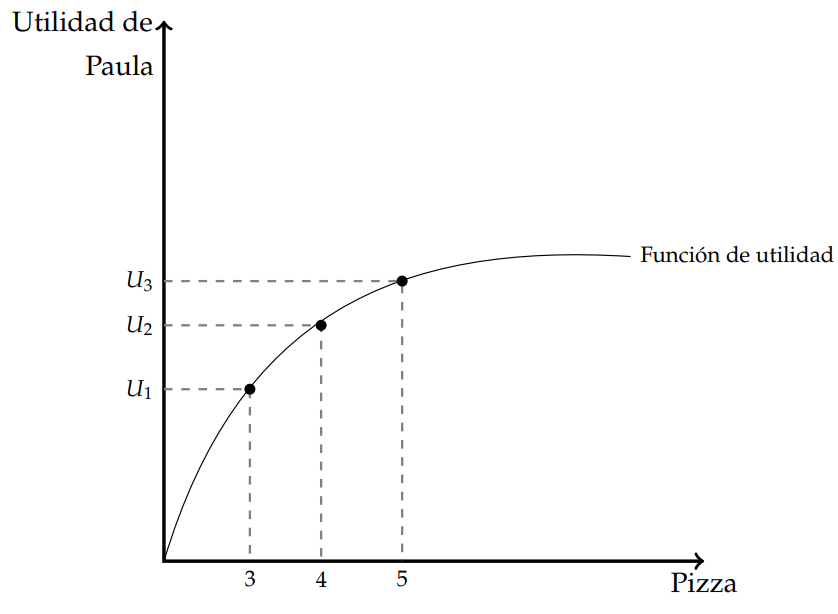
\includegraphics[scale=0.3]{../Figures/C7.9b.png}
\end{center}
\end{frame}

\begin{frame}
\frametitle{Tasa Marginal de Sustitución}
\begin{itemize}
    \item Lo que estoy dispuesto a sacrificar para beneficiarme de una unidad adicional de un bien va cambiando a lo largo de la curva de indiferencia.
    \item La pendiente de la curva de indiferencia describe esa relacion: es la tasa marginal de sustitución
\end{itemize} 
\centering
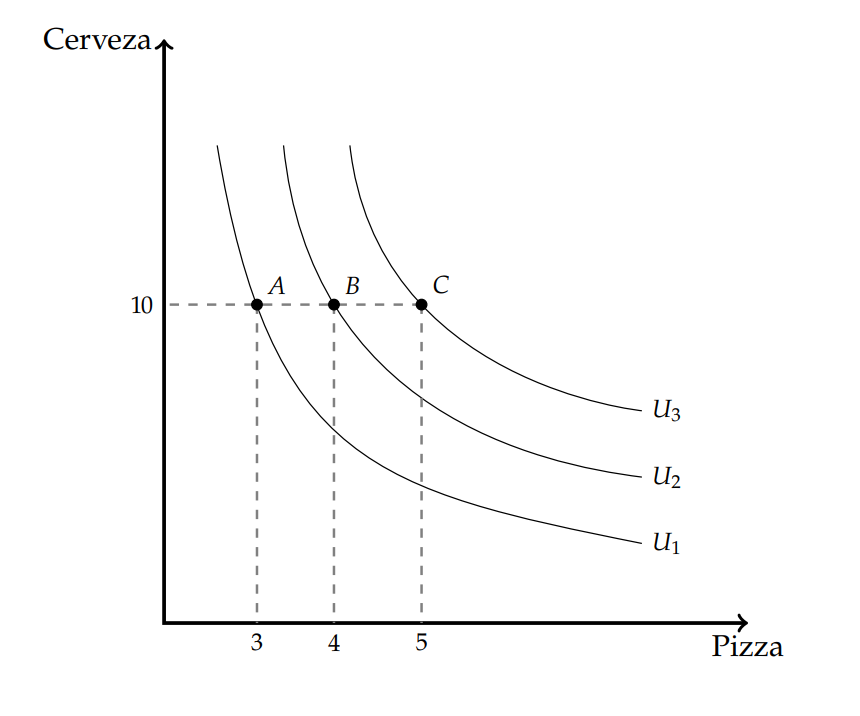
\includegraphics[scale=0.5]{../Figures/C7.9.png}
\end{frame}

\begin{frame}{Tasa Marginal de Sustitución}
    \begin{itemize}
        \item La TMS es la cantidad de unidades de un bien que el individuo está \textbf{dispuesto} a sacrificar a cambio de una unidad adicional del otro bien, de tal manera que se mantiene constante su nivel de utilidad.
        \item Es la pendiente de las curvas de indiferencia:
        \begin{align*}
            \Delta U &= 0 \\
            \Delta U = UMg_x \cdot \Delta X &+ UMg_y \cdot \Delta Y = 0 \\
            UMg_x \cdot \Delta X &= UMg_y \cdot - \Delta Y \\
            TMS = \frac{\Delta Y}{\Delta X} &= - \frac{UMg_x}{UMg_y}
        \end{align*}    
        \item Intuitivamente, nos indica cuántos porrones de cerveza ($Y$) estamos dispuestos a sacrificar a cambio de consumir una porción adicional de pizza ($X$).
        \item ¡No es constante!
    \end{itemize} 
\end{frame}

\begin{frame}
    \frametitle{Bonus: Las curvas de indiferencias pueden tener formas diferentes}
    \begin{columns}
        \column{0.55\textwidth}
        \begin{itemize}
            \item Bienes sustitutos perfectos
            \item Bienes complementarios perfectos
            \item Bien y mal
            \item Bien neutral
        \end{itemize}
        \column{0.5\textwidth}
        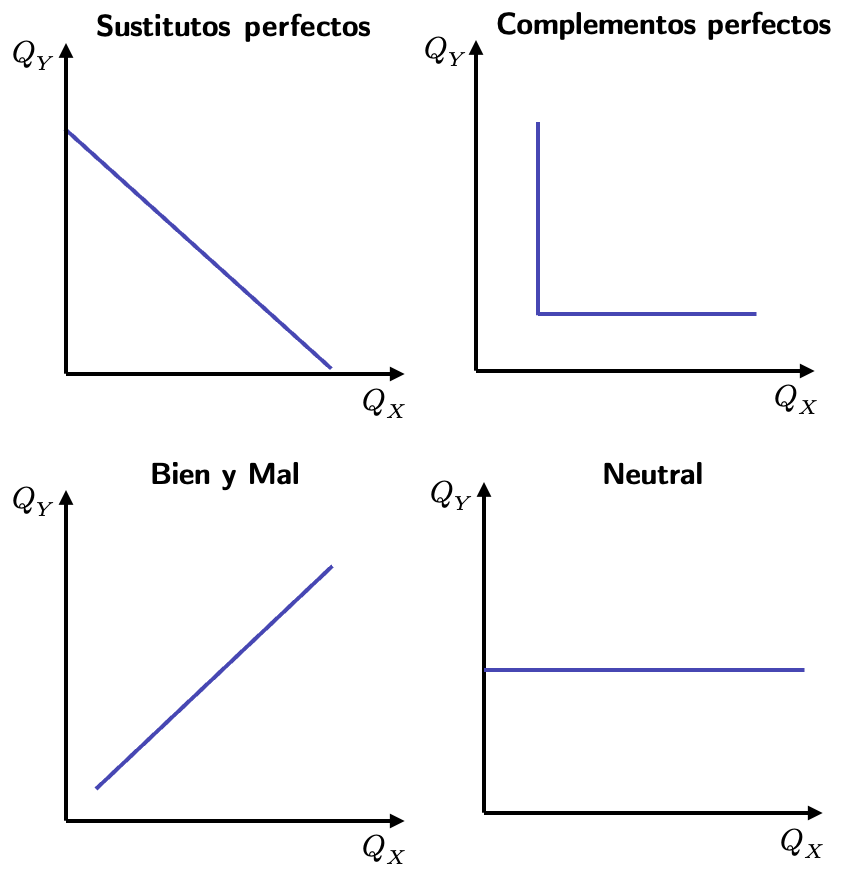
\includegraphics[scale=0.35]{../Figures/CI_casos.png}
    \end{columns}
\end{frame}

\begin{frame}{Comportamiento del consumidor}
    \begin{itemize}
        \item Se puede ver entonces a los consumidores como individuos que tienen: \vspace{-2mm}
        \begin{itemize}
            \item[1.] \textbf{Recursos limitados}. Por lo tanto, enfrentan una restricción presupuestaria. Solo puede elegir entre las canastas de consumo alcanzables
            para él.
            \item[2.] Ciertas \textbf{preferencias} sobre diferentes productos. Para elegir la canasta que más le gusta, debe tener en cuenta
            sus preferencias.
        \end{itemize}
        \item También hacemos un supuesto adicional:
        \begin{itemize}
        \item Los individuos son \textbf{racionales}: toman la mejor decisión posible dada la información.
        \end{itemize}
    \end{itemize} 
\end{frame}

\begin{frame}
    \frametitle{Volviendo al problema del estudiante:}
    \begin{center}
        \begin{tikzpicture}[scale=1.2]
            \node at (3,3) {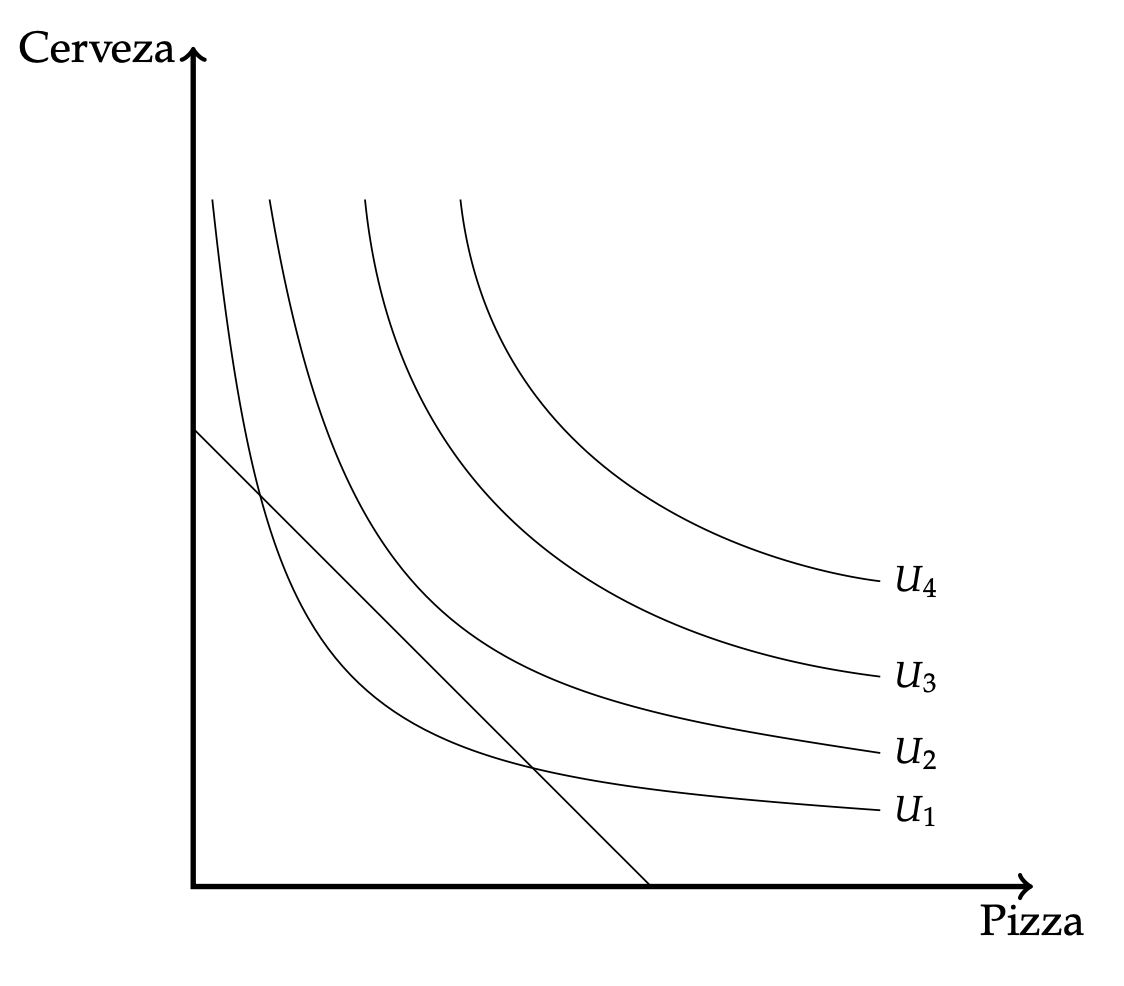
\includegraphics[width=8.5cm]{../Figures/problema_consumidor.png}};
            \node[right] at (-1.8,2.5) {\textbf{Restricción }};
            \node[right] at (-1.8,2) {\textbf{presupuestaria}};
            \draw[->] (0.5,2) -- (2,2);
            \node[above] at (5,3.5) {\textbf{Curvas de indiferencia}};
            \draw[->] (5,3.4) -- (4.5,3);
        \end{tikzpicture}
    \end{center}
\end{frame}

\begin{frame}{Maximizando la utilidad}
    \begin{itemize}
        \item Una idea central en economía es que las personas buscan maximizar su felicidad. \vspace{2mm}
        \begin{itemize}
        \item En la jerga se dice que los individuos intentan ``maximizar su utilidad''. \vspace{2mm}
        \item Pero no nos olvidemos que los individuos enfrentan una restricción presupuestaria. \vspace{2mm}
        \end{itemize} 
        \item Entonces, la pregunta central es: ¿cuál es la mayor utilidad que se puede alcanzar dada la restricción presupuestaria? \vspace{2mm}
        \begin{itemize}
        \item Nos estamos preguntando por la canasta situada en la curva de indiferencia más alta que, al mismo tiempo, sea una de las canastas factibles. 
        \vspace{2mm}
        \end{itemize} 
        \begin{boxB}
        \centering La elección del individuo se basa en maximizar su utilidad sujeto a la restricción presupuestaria
        \end{boxB}
        \end{itemize}
\end{frame}

\begin{frame}
    \frametitle{Equilibrio}
    \begin{center}
        \begin{tikzpicture}[scale=1.2]
            \node at (3,3) {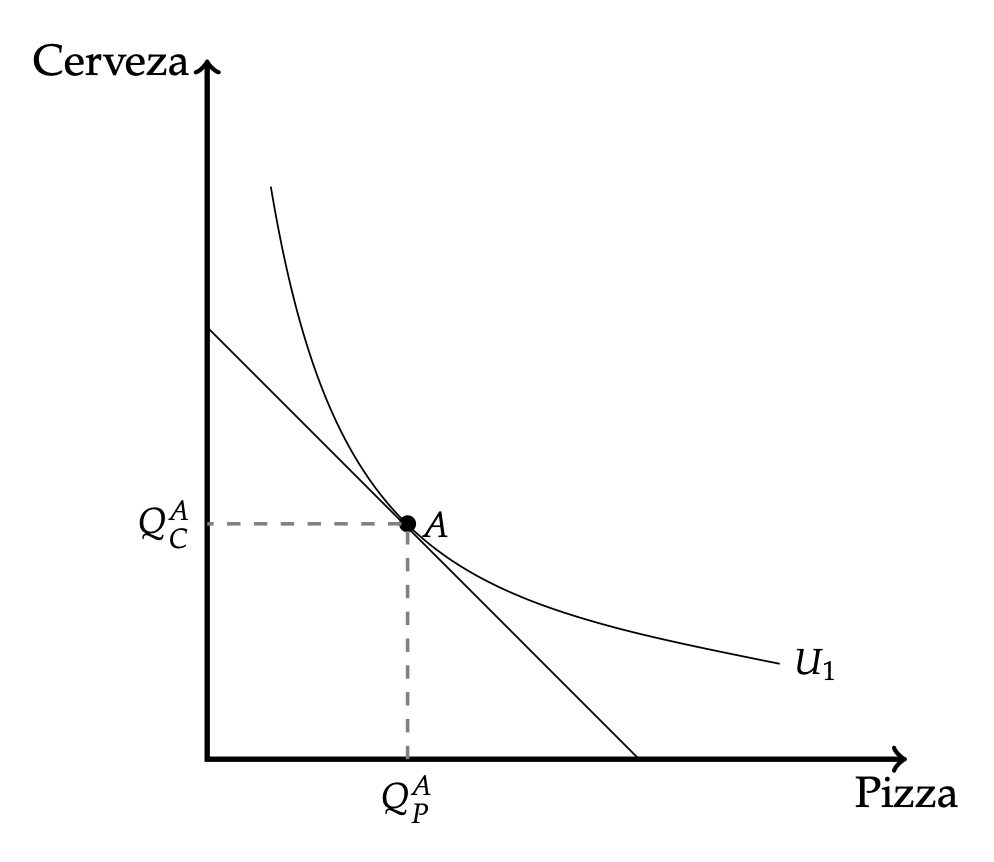
\includegraphics[width=8.5cm]{../Figures/equilibrio.png}};
            \node[above] at (3.5,3) {\textbf{Equilibrio}};
            \draw[->] (3,3) -- (2.5,2.5);
        \end{tikzpicture}
    \end{center}
\end{frame}

\begin{frame}
\frametitle{¿Por qué B no es el punto donde se maximiza la utilidad?}
\centering
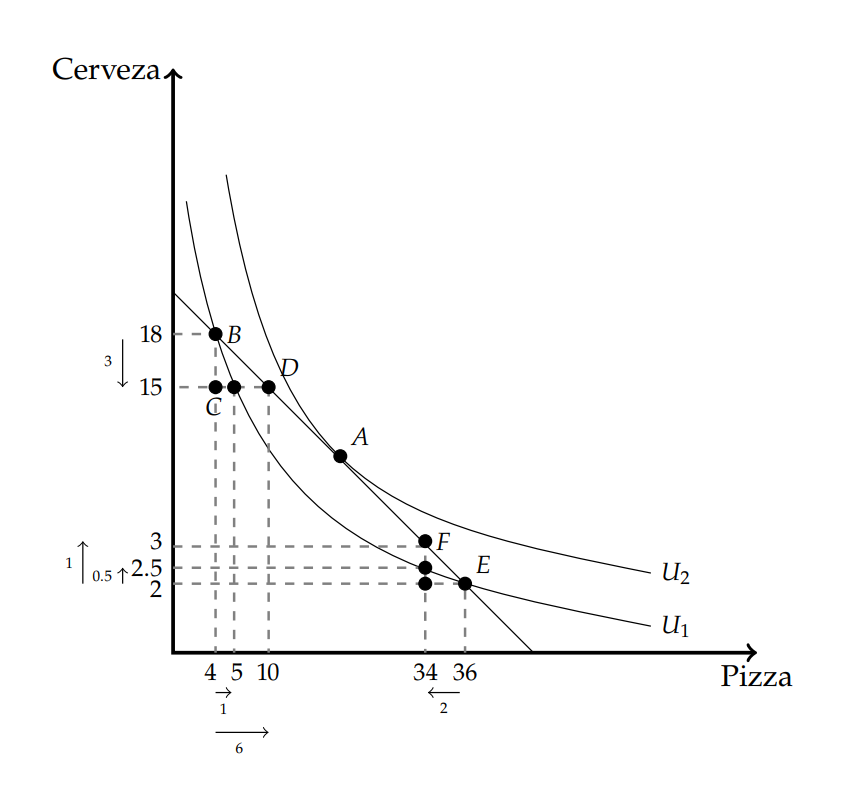
\includegraphics[scale=0.6]{../Figures/C8.3.png}
\end{frame}

\begin{frame}{Resumiendo como decide el consumidor}
    \begin{itemize}
        \item La TMS es la pendiente de la curva de indiferencia y representa la cantidad de bien Y que el consumidor está dispuesto a sacrificar por una unidad adicional del bien X de manera tal que se mantenga constante la utilidad constante
        \[TMS = - \frac{UMg_x}{UMg_y}\]
        \item La TMT es la pendiente de la restricción presupuestaria y muestra la relación a la cual el mercado le permite al consumidor cambiar un producto por el otro
        \[TMT = - \frac{P_x}{P_y}\]
        \item Si $TMS > TMT$, el consumidor está dispuesto a sacrificar más bien Y por una unidad adicional de bien X que lo que el mercado le pide por esa unidad adicional de bien X
        \item La canasta óptima es aquella en la que la TMS es igual a la TMT
    \end{itemize}
\end{frame}

\begin{frame}
\frametitle{Respuesta a shocks (ceteris paribus)}
\begin{itemize}
    \item Queremos ver qué sucede con la decisión del individuo cuando se producen distintos shocks. \vspace{2mm}
    \item Vamos a pensar este shock siguiendo este orden lógico:
    \begin{itemize}
        \item Partiremos de un equilibrio
        \item Propondremos un shock sobre una variable pero el resto de las variables se mantendrán constantes (ceteris paribus)
        \item Discutiremos cómo impacta el shock en la restricción presupuestaria.      
        \item Discutiremos cómo impacta el cambio en la restricción a la decisión de consumo del individuo
    \end{itemize}
\end{itemize} 
\end{frame}

\begin{frame}
\frametitle{Partimos de un equilibrio:}
\begin{center}
\begin{figure}[H]
\renewcommand{\figurename}{Figure}
\begin{center}
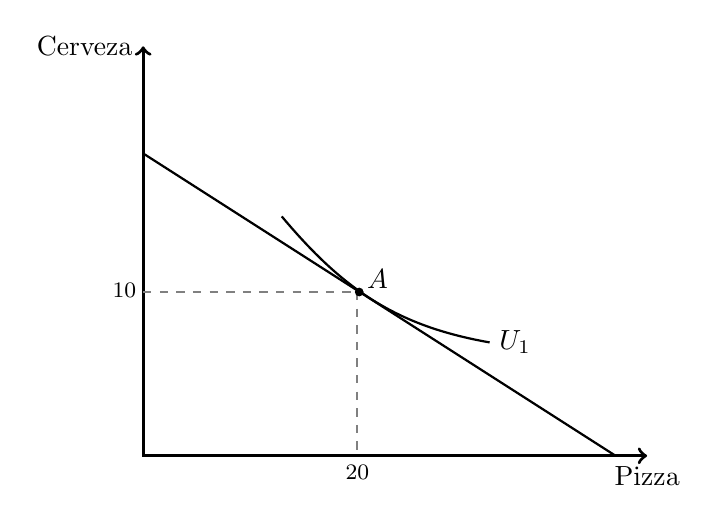
\begin{tikzpicture}[scale=0.8]
\draw[very thick,<->] (0,6.5) node[left]{Cerveza}--(0,0)--(8,0) node[below]{Pizza};
\draw [thick] (2.2,3.8) to [out=310,in=170] (5.5,1.8);
\node [right] at (5.5,1.8) {$U_1$};
\draw[thick, dashed,gray](0,2.6)--(3.4,2.6);
\node[below] at (-0.3,2.9) {\footnotesize 10};
\node[below] at (3.4,0) {\footnotesize 20};
\draw [thick] (0,4.8) -- (7.5,0);
\draw[thick, dashed,gray](3.4,2.6)--(3.4,0);
\node [right] at (3.4,2.8) {$A$};
\draw[fill] (3.43,2.6) circle [radius =0.06];
\end{tikzpicture}
\end{center}
\end{figure}
\end{center}
\end{frame}

\begin{frame}
\frametitle{Cuando hay un shock en el ingreso}
\begin{itemize}
    \item Ceteris paribus: manteniendo todo lo demás constante.
    \item La restricción presupuestaria se desplaza de manera paralela hacia la derecha (con aumento de ingreso) o hacia la izquierda (con disminución de ingreso).
    \item El consumidor va a tener un conjunto factible diferente.
    \item El cambio en el ingreso no altera los precios relativos.
    \item Habrá una nueva canasta óptima para el consumidor, que dependerá de las preferencias del individuo por los bienes en cuestión, es decir, de la forma que presenten las curvas de indiferencia contenidas en el mapa de indiferencia
\end{itemize}
\end{frame}

\begin{frame}{Cuando aumentan las cantidades demandadas (bienes normales)}
    \centering
    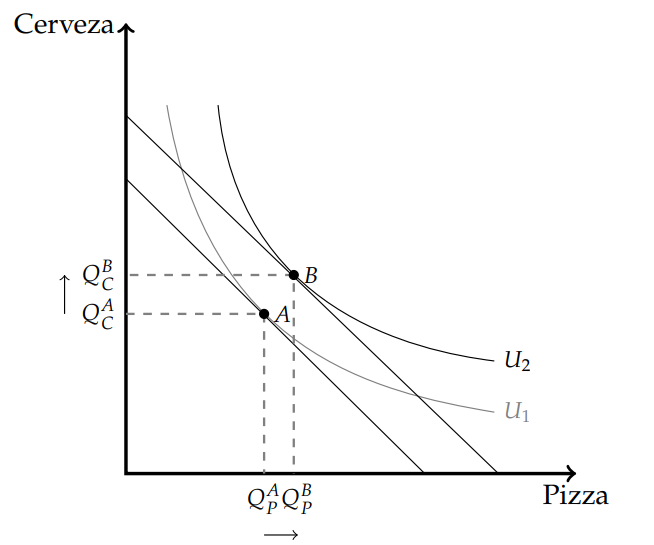
\includegraphics[scale=0.5]{../Figures/C.8.4.png}
\end{frame}

\begin{frame}{Cuando disminuyen las cantidades demandadas (bienes inferiores)}
    \centering
    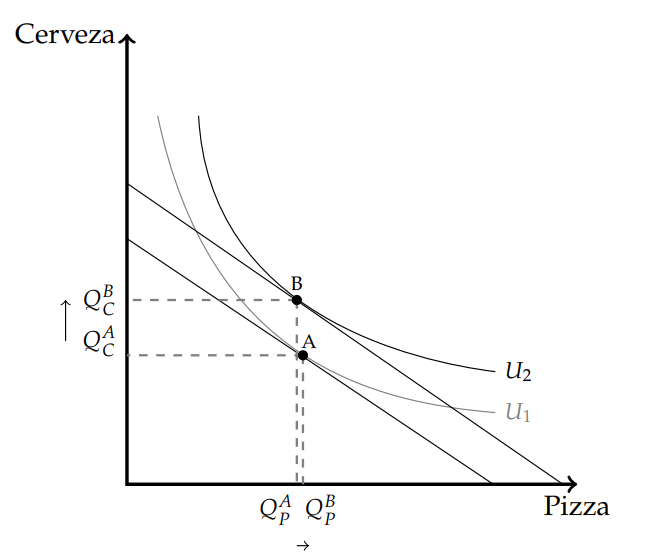
\includegraphics[scale=0.5]{../Figures/C.8.5.png}
\end{frame}

\begin{frame}{Cuando se mantienen constantes las cantidades demandadas (bienes neutrales)}
    \centering
    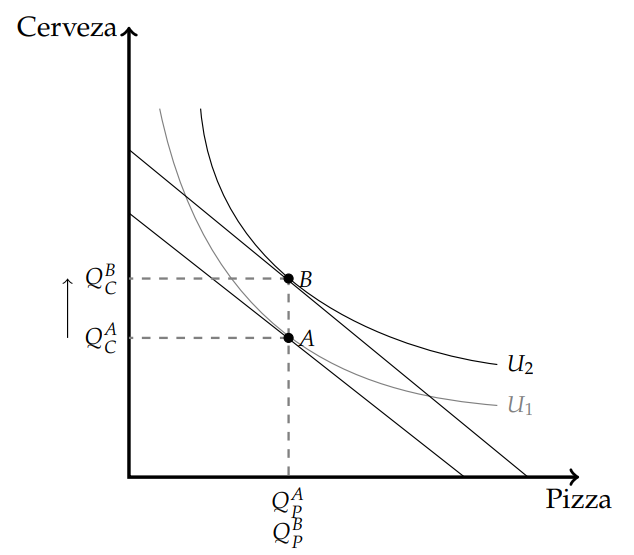
\includegraphics[scale=0.5]{../Figures/C.8.6.png}
\end{frame}

\begin{frame}
\frametitle{Cuando hay un shock en el precio de un bien}
\begin{itemize}
    \item Ceteris paribus: manteniendo todo lo demás constante.
    \item La restricción presupuestaria pivotea sobre el bien que no cambia el precio, reduciendo (aumentando) la cantidad máxima del bien afectado por el aumento (disminución) del precio.  
    \item El consumidor va a tener menos (más) canastas disponibles porque su conjunto factible se ha reducido (expandido).
    \item El cambio en el precio de un bien también altera los precios relativos. 
    \item Habrá una nueva canasta óptima para el consumidor.
\end{itemize}
\end{frame}

\begin{frame}
\frametitle{¿Cuál es el efecto total de un aumento en el precio de la pizza? Partimos del equilibrio A}
\begin{center}
\begin{figure}[H]
\renewcommand{\figurename}{Figure}
\begin{center}
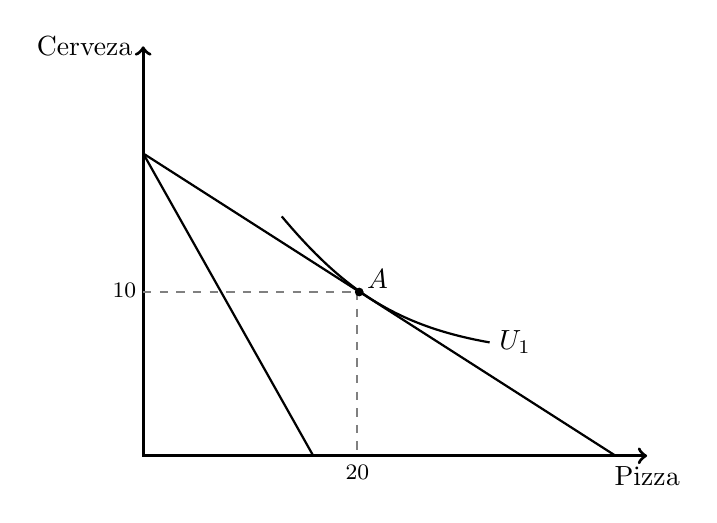
\begin{tikzpicture}[scale=0.8]
\draw[very thick,<->] (0,6.5) node[left]{Cerveza}--(0,0)--(8,0) node[below]{Pizza};
\draw [thick] (2.2,3.8) to [out=310,in=170] (5.5,1.8);
\node [right] at (5.5,1.8) {$U_1$};
\node[below] at (3.4,0) {\footnotesize 20};
\draw [thick] (0,4.8) -- (7.5,0);
\draw [thick] (0,4.8) -- (2.7,0);
\draw[thick, dashed,gray](0,2.6)--(3.4,2.6);
\node[below] at (-0.3,2.9) {\footnotesize 10};
\draw[thick, dashed,gray](3.4,2.6)--(3.4,0);
\node [right] at (3.4,2.8) {$A$};
\draw[fill] (3.43,2.6) circle [radius =0.06];
\end{tikzpicture}
\end{center}
\end{figure}
\end{center}
\end{frame}

\begin{frame}
\frametitle{La nueva canasta óptima es B}
\begin{center}
\begin{figure}[H]
\renewcommand{\figurename}{Figure}
\begin{center}
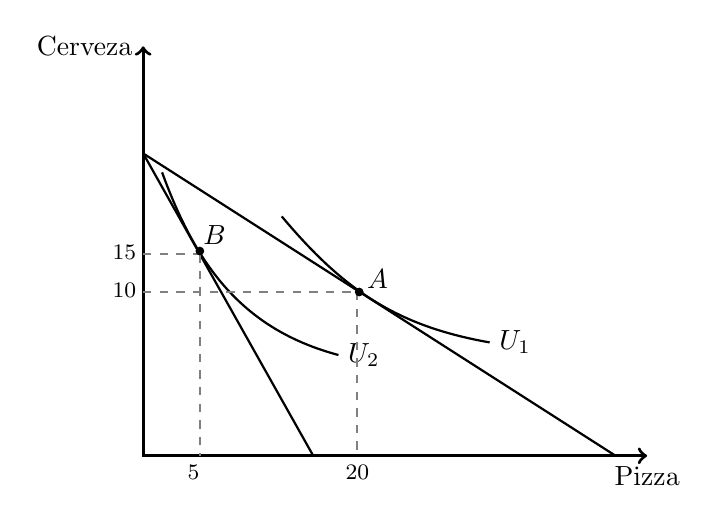
\begin{tikzpicture}[scale=0.8]
\draw[very thick,<->] (0,6.5) node[left]{Cerveza}--(0,0)--(8,0) node[below]{Pizza};
\draw [thick] (2.2,3.8) to [out=310,in=170] (5.5,1.8);
\node [right] at (5.5,1.8) {$U_1$};
\draw [thick] (0.3,4.5) to [out=290,in=165] (3.1,1.6);
\node [right] at (3.1,1.6) {$U_2$};
\node[below] at (3.4,0) {\footnotesize 20};
\node[below] at (0.8,0) {\footnotesize 5};
\draw [thick] (0,4.8) -- (7.5,0);
\draw [thick] (0,4.8) -- (2.7,0);
\draw[thick, dashed,gray](0.9,3.2)--(0.9,0);
\draw[thick, dashed,gray](0,3.2)--(0.9,3.2);
\node[below] at (-0.3,3.5) {\footnotesize 15};
\draw[thick, dashed,gray](0,2.6)--(3.4,2.6);
\node[below] at (-0.3,2.9) {\footnotesize 10};
\draw[thick, dashed,gray](3.4,2.6)--(3.4,0);
\node [right] at (0.8,3.5) {$B$};
\draw[fill] (0.9,3.25) circle [radius =0.06];
\node [right] at (3.4,2.8) {$A$};
\draw[fill] (3.43,2.6) circle [radius =0.06];
\end{tikzpicture}
\end{center}
\end{figure}
\end{center}
\end{frame}

\begin{frame}
\frametitle{El efecto total de un aumento en el precio de la Pizza} 
\begin{center}
\begin{figure}[H]
\renewcommand{\figurename}{Figure}
\begin{center}
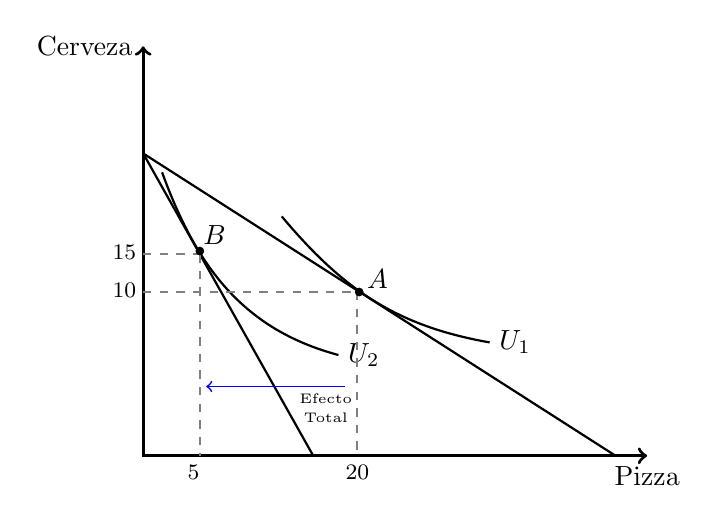
\begin{tikzpicture}[scale=0.8]
\draw[very thick,<->] (0,6.5) node[left]{Cerveza}--(0,0)--(8,0) node[below]{Pizza};
\draw [thick] (2.2,3.8) to [out=310,in=170] (5.5,1.8);
\node [right] at (5.5,1.8) {$U_1$};
\draw [thick] (0.3,4.5) to [out=290,in=165] (3.1,1.6);
\node [right] at (3.1,1.6) {$U_2$};
\node[below] at (3.4,0) {\footnotesize 20};
\node[below] at (0.8,0) {\footnotesize 5};
\draw [thick] (0,4.8) -- (7.5,0);
\draw [thick] (0,4.8) -- (2.7,0);
\draw[thick, dashed,gray](0.9,3.2)--(0.9,0);
\draw[thick, dashed,gray](3.4,2.6)--(3.4,0);
\draw[semithick, blue, <-] (1,1.1)--(3.2,1.1);
\draw[thick, dashed,gray](0,3.2)--(0.9,3.2);
\node[below] at (-0.3,3.5) {\footnotesize 15};
\draw[thick, dashed,gray](0,2.6)--(3.4,2.6);
\node[below] at (-0.3,2.9) {\footnotesize 10};
\node[] at (2.9,0.9){\tiny Efecto};
\node[] at (2.9,0.6){\tiny Total};
\node [right] at (0.8,3.5) {$B$};
\draw[fill] (0.9,3.25) circle [radius =0.06];
\node [right] at (3.4,2.8) {$A$};
\draw[fill] (3.43,2.6) circle [radius =0.06];
\end{tikzpicture}
\end{center}
\end{figure}
\end{center}
\end{frame}

\begin{frame}
\frametitle{El efecto ingreso y el efecto sustitución}
\begin{itemize}
    \item Un aumento en el precio de la pizza produce dos efectos:
    \begin{itemize}
        \item Disminuye el poder de compra, porque el consumidor tiene menor poder adquisitivo.
        \item Aumenta el costo de oportunidad de la pizza, porque el precio relativo de la pizza ha aumentado (ahora es una cerveza entera!).
    \end{itemize}
    \item \textbf{Efecto ingreso}: El efecto que el ingreso menor tendría si no hubiera cambios en el costo de oportunidad
    \begin{itemize}
        \item Gráficamente, ``es como'' si la restricción se desplazara hacia adentro.
    \end{itemize}
    
    \item \textbf{Efecto sustitución}: El efecto del cambio en el costo de oportunidad, porque cambiaron los precios relativos (aumentó la TMT, o sea la pendiente de la RP).
\end{itemize} 
\end{frame}

\begin{frame}
\frametitle{Y si le damos menos dinero para que esté sobre $U_2$, ¿elige B?}
\begin{center}
\begin{figure}[H]
\renewcommand{\figurename}{Figure}
\begin{center}
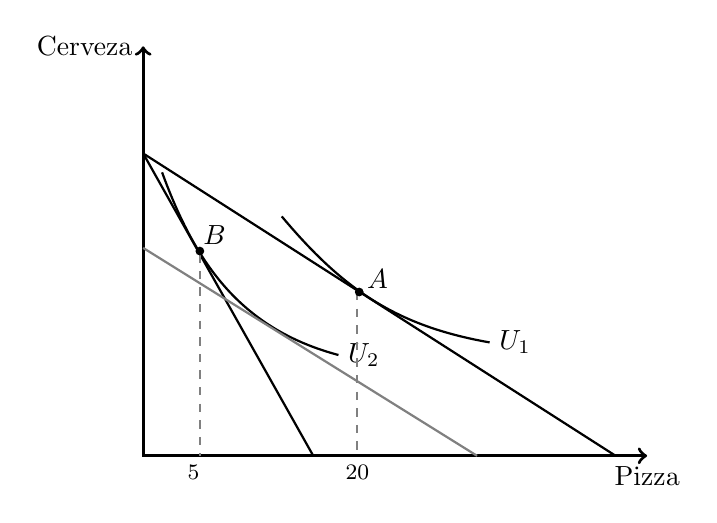
\begin{tikzpicture}[scale=0.8]
\draw[very thick,<->] (0,6.5) node[left]{Cerveza}--(0,0)--(8,0) node[below]{Pizza};
\draw [thick] (2.2,3.8) to [out=310,in=170] (5.5,1.8);
\node [right] at (5.5,1.8) {$U_1$};
\draw [thick] (0.3,4.5) to [out=290,in=165] (3.1,1.6);
\node [right] at (3.1,1.6) {$U_2$};
\node[below] at (3.4,0) {\footnotesize 20};
\node[below] at (0.8,0) {\footnotesize 5};
\draw [thick] (0,4.8) -- (7.5,0);
\draw [thick] (0,4.8) -- (2.7,0);
\draw[thick, dashed,gray](0.9,3.2)--(0.9,0);
\draw[thick, dashed,gray](3.4,2.6)--(3.4,0);
\draw [thick, gray] (0,3.3) -- (5.3,0);
\node [right] at (0.8,3.5) {$B$};
\draw[fill] (0.9,3.25) circle [radius =0.06];
\node [right] at (3.4,2.8) {$A$};
\draw[fill] (3.43,2.6) circle [radius =0.06];
\end{tikzpicture}
\end{center}

\end{figure}
\end{center}
\end{frame}


\begin{frame}
\frametitle{No, ¡elige C!}
\begin{center}
\begin{figure}[H]
\renewcommand{\figurename}{Figure}
\begin{center}
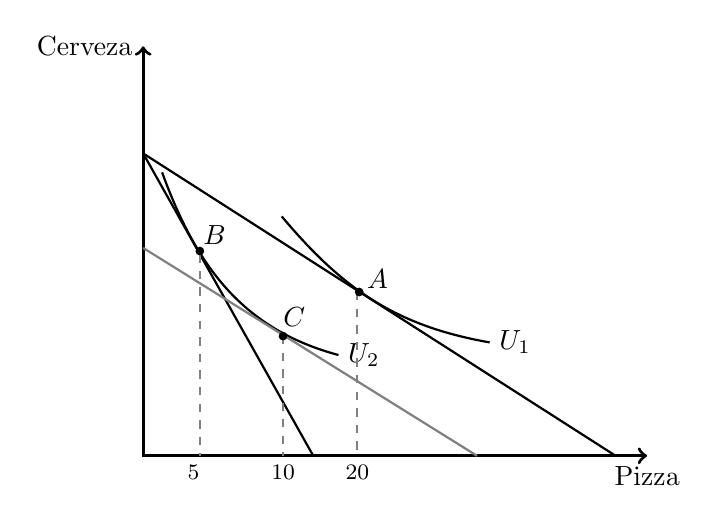
\begin{tikzpicture}[scale=0.8]
\draw[very thick,<->] (0,6.5) node[left]{Cerveza}--(0,0)--(8,0) node[below]{Pizza};
\draw [thick] (2.2,3.8) to [out=310,in=170] (5.5,1.8);
\node [right] at (5.5,1.8) {$U_1$};
\draw [thick] (0.3,4.5) to [out=290,in=165] (3.1,1.6);
\node [right] at (3.1,1.6) {$U_2$};
\node[below] at (3.4,0) {\footnotesize 20};
\node[below] at (2.22,0) {\footnotesize 10};
\node[below] at (0.8,0) {\footnotesize 5};
\draw [thick] (0,4.8) -- (7.5,0);
\draw [thick] (0,4.8) -- (2.7,0);
\draw[thick, dashed,gray](0.9,3.2)--(0.9,0);
\draw[thick, dashed,gray](3.4,2.6)--(3.4,0);
\draw[thick, dashed,gray](2.22,1.9)--(2.22,0);
\draw [thick, gray] (0,3.3) -- (5.3,0);
\node [above] at (2.4,1.9) {$C$};
\draw[fill] (2.22,1.9) circle [radius =0.06];
\node [right] at (0.8,3.5) {$B$};
\draw[fill] (0.9,3.25) circle [radius =0.06];
\node [right] at (3.4,2.8) {$A$};
\draw[fill] (3.43,2.6) circle [radius =0.06];
\end{tikzpicture}
\end{center}

\end{figure}
\end{center}
\end{frame}

\begin{frame}
\frametitle{El efecto ingreso}
\begin{center}
\begin{figure}[H]
\renewcommand{\figurename}{Figure}
\begin{center}
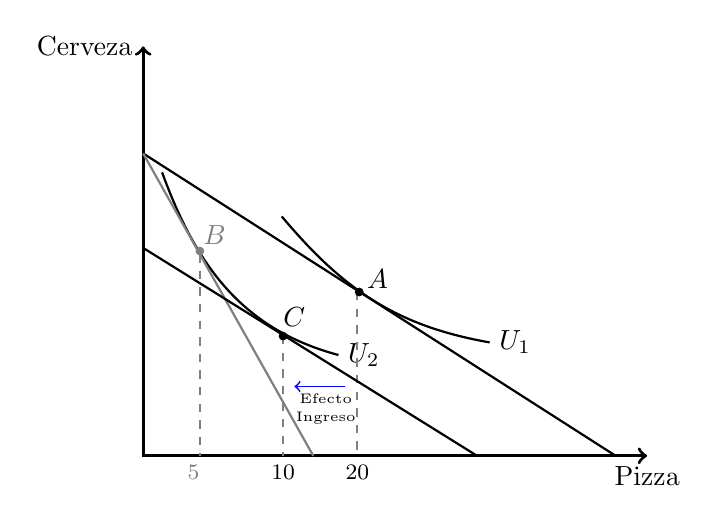
\begin{tikzpicture}[scale=0.8]
\draw[very thick,<->] (0,6.5) node[left]{Cerveza}--(0,0)--(8,0) node[below]{Pizza};
\draw [thick] (2.2,3.8) to [out=310,in=170] (5.5,1.8);
\node [right] at (5.5,1.8) {$U_1$};
\draw [thick] (0.3,4.5) to [out=290,in=165] (3.1,1.6);
\node [right] at (3.1,1.6) {$U_2$};
\node[below] at (3.4,0) {\footnotesize 20};
\node[below] at (2.22,0) {\footnotesize 10};
\node[below,gray] at (0.8,0) {\footnotesize 5};
\draw [thick] (0,4.8) -- (7.5,0);
\draw [thick,gray] (0,4.8) -- (2.7,0);
\draw[thick, dashed,gray](0.9,3.2)--(0.9,0);
\draw[thick, dashed,gray](3.4,2.6)--(3.4,0);
\draw[thick, dashed,gray](2.22,1.9)--(2.22,0);
\draw [thick] (0,3.3) -- (5.3,0);
\draw[semithick, blue, <-] (2.4,1.1)--(3.2,1.1);
\node[] at (2.9,0.9){\tiny Efecto};
\node[] at (2.9,0.6){\tiny Ingreso};
\node [above] at (2.4,1.9) {$C$};
\draw[fill] (2.22,1.9) circle [radius =0.06];
\node [right,gray] at (0.8,3.5) {$B$};
\draw[fill,gray] (0.9,3.25) circle [radius =0.06];
\node [right] at (3.4,2.8) {$A$};
\draw[fill] (3.43,2.6) circle [radius =0.06];
\end{tikzpicture}
\end{center}
\end{figure}
\end{center}
\end{frame}

\begin{frame}
\frametitle{El efecto sustitución}
\begin{center}
\begin{figure}[H]
\renewcommand{\figurename}{Figure}
\begin{center}
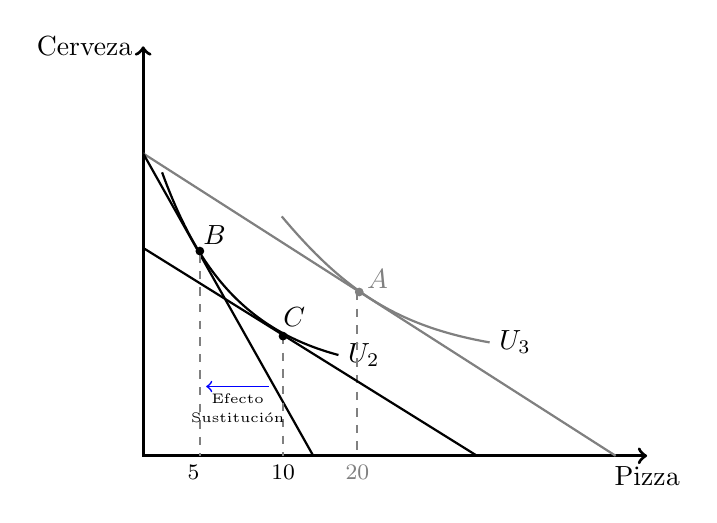
\begin{tikzpicture}[scale=0.8]
\draw[very thick,<->] (0,6.5) node[left]{Cerveza}--(0,0)--(8,0) node[below]{Pizza};
\draw [thick,gray] (2.2,3.8) to [out=310,in=170] (5.5,1.8);
\node [right] at (5.5,1.8) {$U_3$};
\draw [thick] (0.3,4.5) to [out=290,in=165] (3.1,1.6);
\node [right] at (3.1,1.6) {$U_2$};
\node[below,gray] at (3.4,0) {\footnotesize 20};
\node[below] at (2.22,0) {\footnotesize 10};
\node[below] at (0.8,0) {\footnotesize 5};
\draw [thick,gray] (0,4.8) -- (7.5,0);
\draw [thick] (0,4.8) -- (2.7,0);
\draw[thick, dashed,gray](0.9,3.2)--(0.9,0);
\draw[thick, dashed,gray](3.4,2.6)--(3.4,0);
\draw[thick, dashed,gray](2.22,1.9)--(2.22,0);
\draw [thick] (0,3.3) -- (5.3,0);
\draw[semithick, blue, <-] (1,1.1)--(2,1.1);
\node[] at (1.5,0.9){\tiny Efecto};
\node[] at (1.5,0.6){\tiny Sustitución};
\node [above] at (2.4,1.9) {$C$};
\draw[fill] (2.22,1.9) circle [radius =0.06];
\node [right] at (0.8,3.5) {$B$};
\draw[fill] (0.9,3.25) circle [radius =0.06];
\node [right,gray] at (3.4,2.8) {$A$};
\draw[fill,gray] (3.43,2.6) circle [radius =0.06];
\end{tikzpicture}
\end{center}
\end{figure}
\end{center}
\end{frame}


\begin{frame}
\frametitle{La suma del efecto sustitución y el efecto ingreso nos da el efecto total}
\begin{center}
\begin{figure}[H]
\renewcommand{\figurename}{Figure}
\begin{center}
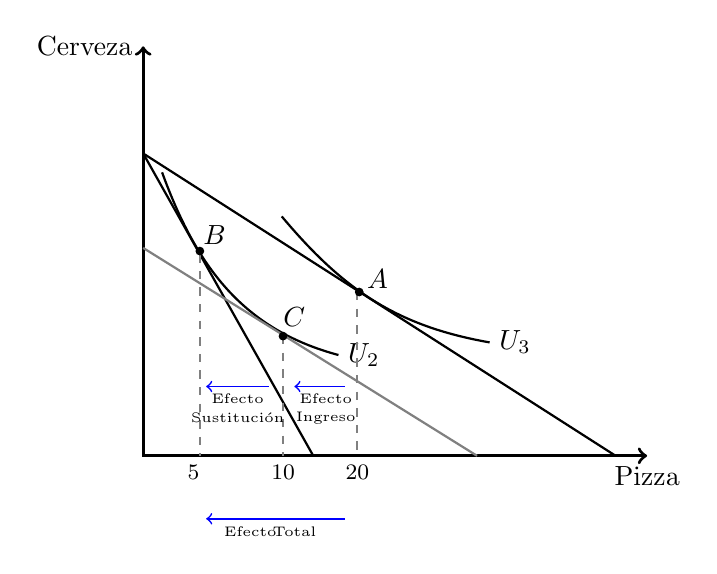
\begin{tikzpicture}[scale=0.8]
\draw[very thick,<->] (0,6.5) node[left]{Cerveza}--(0,0)--(8,0) node[below]{Pizza};
\draw [thick] (2.2,3.8) to [out=310,in=170] (5.5,1.8);
\node [right] at (5.5,1.8) {$U_3$};
\draw [thick] (0.3,4.5) to [out=290,in=165] (3.1,1.6);
\node [right] at (3.1,1.6) {$U_2$};
\node[below] at (3.4,0) {\footnotesize 20};
\node[below] at (2.22,0) {\footnotesize 10};
\node[below] at (0.8,0) {\footnotesize 5};
\draw [thick] (0,4.8) -- (7.5,0);
\draw [thick] (0,4.8) -- (2.7,0);
\draw[thick, dashed,gray](0.9,3.2)--(0.9,0);
\draw[thick, dashed,gray](3.4,2.6)--(3.4,0);
\draw[thick, dashed,gray](2.22,1.9)--(2.22,0);
\draw [thick, gray] (0,3.3) -- (5.3,0);
\draw[semithick, blue, <-] (1,-1)--(3.2,-1);
\node[] at (1.7,-1.2){\tiny Efecto};
\node[] at (2.4,-1.2){\tiny Total};
\draw[semithick, blue, <-] (2.4,1.1)--(3.2,1.1);
\node[] at (2.9,0.9){\tiny Efecto};
\node[] at (2.9,0.6){\tiny Ingreso};
\draw[semithick, blue, <-] (1,1.1)--(2,1.1);
\node[] at (1.5,0.9){\tiny Efecto};
\node[] at (1.5,0.6){\tiny Sustitución};
\node [above] at (2.4,1.9) {$C$};
\draw[fill] (2.22,1.9) circle [radius =0.06];
\node [right] at (0.8,3.5) {$B$};
\draw[fill] (0.9,3.25) circle [radius =0.06];
\node [right] at (3.4,2.8) {$A$};
\draw[fill] (3.43,2.6) circle [radius =0.06];
\end{tikzpicture}
\end{center}
\end{figure}
\end{center}
\end{frame}

\end{document}

